\documentclass[dvipsnames]{beamer}
\setbeamertemplate{navigation symbols}{} % suppresses all navigation symbols
\usepackage{sidebarStyle}
\linespread{1.3} % line spacing of 1.5
\usepackage[T1]{fontenc}
\usepackage[utf8]{inputenc}
\usepackage[english]{babel}
\usepackage[babel]{csquotes}
% Graphics related packages:
\usepackage{tikz,pgfplots,graphicx,siunitx}
\pgfplotsset{compat=1.17}
\DeclareSIUnit\torr{torr}
\usepackage[mode=buildnew]{standalone}
\usepackage{tikzscale}
\usepackage{ifthen} % used in fiber.tikz
\usetikzlibrary{calc} % used in fiber.tikz
\usetikzlibrary{math} % used in starkBroadening.tikz
\usepgfplotslibrary{units}
\usepgfplotslibrary{fillbetween} % used in sample_lorentzian.tikz
\pgfplotsset{every axis/.append style={line join=round, line cap=round}}

%% To reduce compilation time
\usepgfplotslibrary{external}
\tikzexternalize[prefix=tikz/,optimize command away=\pdfpages]
\usepackage{pdfpages} % To include pdf pages
\usepackage{adjustbox} % for \adjincludegraphics for begin{columns}
\setbeamertemplate{caption}{\raggedleft\insertcaption\par} % To remove figure caption prefix “figure”

%Information to be included in the title page:
\title[]{Low jitter plasma channel in 3D printed gas filled capillary discharges}
\subtitle{Thesis Presentation}
\author[]{Ehud Behar}
\institute{Hebrew University of Jerusalem}
\date{2021}
\logo{\includegraphics[width=10mm]{figures/logo}}

\AtBeginSection[]
{
  \begin{frame}
    \frametitle{Table of Contents}
    \tableofcontents[currentsection]
  \end{frame}
} % put the table of contents at the beginning of each section and highlight the title of the current section
% \AtBeginSubsection[] {
%     \begin{frame}<beamer>{Table of Contents}
%     \tableofcontents[currentsection,currentsubsection]
%     \end{frame}
% }
% from https://tex.stackexchange.com/a/415653/180429
%\setbeamertemplate{frametitle continuation}{\insertcontinuationcount}
\begin{document}

\frame{\titlepage}
% \begin{frame}
% \frametitle{Table of Contents}
% \tableofcontents
% \end{frame}

\section{Background}
\subsection{Introduction}
  \begin{frame}{Introduction}
  \begin{center}
    The goal --- design a low--jitter plasma channel for a table--top particle accelerator.
  \end{center}
    Applications:
    \begin{itemize}
        \item[\textbullet] Experiments on the structure of matter
        \item[\textbullet] Creating radiation sources
        \item[\textbullet] Treatment of cancer
    \end{itemize}
  \end{frame}

\begin{frame}{Linear accelerators}
At present, all high energy accelerators run into limits.
\begin{itemize}
\item[\textbullet] The acclerating electric fields must be less than \SI[per-mode=symbol]{100}{\mega \V \per\meter}, to avoid material breakdown.
\item[\textbullet] Each \si{\giga \eV} of energy requires $\sim$\SI{100}{\meter} of accleration length.
\end{itemize}
\begin{figure}
\includegraphics[width=200pt]{figures/theory/lhc_cern_compressed.jpg}
\end{figure}
\end{frame}
\begin{frame}{Laser Wake--Field Acceleration --- LWFA}{A plasma--based chraged particles accelerator}
Electrical breakdown is part of the design.

The power source is a laser beam or a charged particle beam.
\tikzsetnextfilename{lwfa-schematic}
\begin{figure}
\includegraphics[width=300pt,height=150pt]{figures/theory/lwfa-schematic.tikz}
\end{figure}
\end{frame}

\begin{frame}{LWFA}{Limitations}
Laser defocusing
\tikzsetnextfilename{defocusing}
\begin{figure}
\centering
\includegraphics[width=180pt,height=110pt]{figures/theory/defocusing.tikz}
\end{figure}
Acceleration is achieved only when the laser beam is focused

to $\sim$ tens of \si{\um} in diameter.

Solution: Use a wave--guide.
\end{frame}

\begin{frame}{Waveguide}{Basic concept}
 \tikzsetnextfilename{fiber}
 \begin{figure}
 \includegraphics[width=0.8\textwidth]{figures/theory/fiber.tikz}
  \end{figure}
  Light confined in core, cladding with a smaller refractive index.
\end{frame}
\begin{frame}{Construct a plasma waveguide}{Capillary Discharge}
Generate a plasma channel by means of electrical discharge.
\begin{columns}
\column{0.5\textwidth}
\begin{figure}
 \centering
 \includegraphics[height=130pt]{figures/theory/ablated.png}
 \caption{Ablated capillary}
\end{figure}
\column{0.5\textwidth}
\begin{figure}
\centering
\includegraphics[height=130pt]{figures/theory/gasfilled_with_barb.png}
\caption{Gas–-filled capillary}
\end{figure}
\end{columns}
Apply voltage ($\sim$\si{\kV}) on the capillary ends to start a discharge.
% high-mobility electrons pick up energy from the applied electric field and then transfer part of this  energy to  the heavy particles through elastic collisions. page 4 in Boulos
\end{frame}
\subsection{Background to plasma}
\begin{frame}{The Plasma state}
Ionised gas, electrically neutral.

Defined by $N_e\left(\si{\per\cubic\cm} \right)$ and $T_e\left(\si{\electronvolt} \right)$.

Characteristic quantities:
  \begin{tabular}{l c r}
  Debye length & $\lambda_D=\sqrt{\frac{\varepsilon_0 k_B T_e}{N_e e^2}}$ &  \includegraphics[height=50pt]{figures/theory/white_background.png}\\ 
  Plasma Frequency & $ \omega_p=\sqrt{\frac{N_e e^2}{m_e \varepsilon_0}}\si[per-mode=fraction]{\radian\per\sec} $ & \includegraphics[height=50pt]{figures/theory/white_background.png}\\
  % \onslide<3-> Plasma parameter & $ \Lambda=4\pi N_e \lambda_D ^3 $ & \includegraphics[height=50pt]{figures/theory/white_background.png} \\
  \end{tabular}
\end{frame}

\subsection{Preformed Plasma channel}
\begin{frame}{Parabolic density profile}
 Plasma dispersion relation:
 \begin{equation*}
\omega^2=\omega_p^2+c^2k^2
 \end{equation*}
 The index of refraction $\tilde n$ is
 \begin{equation*}
\tilde{n}=\frac{c k}{\omega}=\sqrt{1-\frac{\omega_p^2}{\omega_L^2}}\approx1-\frac{\omega_p^2}{2\omega_L^2}=1-\frac{N_e}{2N_\text{cr}}
 \end{equation*}
 {\small where
\begin{equation*}
 N_\text{cr}=\frac{\omega_L^2\varepsilon_0 m_e}{e^2}
\end{equation*}
is the critical plasma density.}
\end{frame}
%\begin{frame}{Parabolic density profile}
% To achieve guiding, we need variation in $\tilde{n}$.
%
% Ideally, the radial density profile (RDP) is parabolic:
%\begin{equation*}
%N_e(r)=N_e(0)+\Delta N_e\left( \frac{r}{r_\text{ch}}\right)^2
% \end{equation*}
% \begin{columns}
%  \column{0.5\textwidth}
%  \tikzsetnextfilename{rdp}
%\includegraphics[height=100pt]{figures/theory/rdp.tikz}
%  \column{0.5\textwidth}
%  \tikzsetnextfilename{density_vs_r}
%\includegraphics[height=100pt]{figures/theory/density_vs_r.tikz}
% \end{columns}
%\end{frame}

\subsection{Characterisation of the plasma}
\begin{frame}{Characterisation of the plasma}{Hydrogen Spectrum}
Hot plasma emits light.

The emitted spectra can give information about $N_e$ and $T_e$.
\begin{columns}
\column{0.4\textwidth}
 \tikzsetnextfilename{hydrogenEnergyLevels}
 \includegraphics[width=\textwidth,height=95pt]{figures/theory/hydrogenEnergyLevels.tikz}
\column{0.5\textwidth}
 \includegraphics[width=\textwidth]{figures/theory/purple_plasma.png}
\end{columns}
$$H_{\alpha}:\ \lambda=\SI{656.28}{\nm}
$$
\end{frame}
% \begin{frame}{Plasma spectroscopy}{Electron density measurement}
% Study of the emitted spectra gives information on the plasma.
% \vskip 2em
% \begin{columns}
% \column{0.5\textwidth}
% 
% \column{0.5\textwidth}
% \includegraphics[width=\textwidth]{figures/theory/purple_plasma.png}
% \end{columns}
% \begin{center}
%  \vskip 1em
% plasma diagnostic under a theoretical model --- the LTE model.
% \end{center}
% \end{frame}
% \begin{frame}{Optical Depth}{Optically thin plasma}
%  Optical depth $\tau$ \small{(dimensionless)} --- a measure of the opacity of the medium:
%  \begin{equation*}
% \tau=-\kappa z
%  \end{equation*}
%  $\kappa$ --- the linear absorption coefficient (\si{\per\cm}).
% 
%  $I_\text{out}$ and $I_\text{in}$ are related by
%  \begin{equation*}
% I_\text{out} = I_\text{in}\mathrm{e}^{-\kappa z}
%  \end{equation*}
% \begin{columns}
%  \column{0.4\textwidth}
%  \tikzsetnextfilename{radiativeTransfer}
%   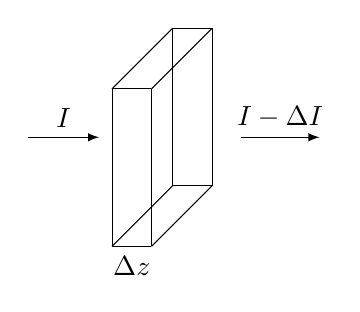
\begin{tikzpicture}
\draw(-0.25,1,1) -- (0.25,1,1);
\draw(-0.25,1,1) -- (-0.25,1,-1);
\draw(-0.25,1,1) -- (-0.25,-1,1);
\draw(0.25,1,1) -- (0.25,1,-1);
\draw(0.25,1,1) -- (0.25,-1,1);
\draw(0.25,1,-1) -- (-0.25,1,-1);
\draw(0.25,1,-1) -- (0.25,-1,-1);
\draw(-0.25,1,-1) -- (-0.25,-1,-1);
\draw(-0.25,-1,1) -- node [midway, below] {$\Delta z$} (0.25,-1,1);
\draw(0.25,-1,-1) -- (0.25,-1,1);
\draw(0.25,-1,-1) -- (-0.25,-1,-1);
\draw(-0.25,-1,-1) -- (-0.25,-1,1);
\draw[-latex] (-1.7,0,0) -- node [midway, above] {$I$} (-0.8,0,0);
\draw[-latex] (1,0,0) --  node [midway, above] {$I-\Delta I$} (2,0,0) ;


\end{tikzpicture}

% \column{0.6\textwidth}
%  \begin{center}
%  \begin{tabular}{ c c c }
% $\tau<1$ & $\longrightarrow$ & optically thin medium\\ 
% $\tau>1$ & $\longrightarrow$ & optically thick medium
%  \end{tabular}
%  \end{center}
% \end{columns}
% \end{frame}
% % \begin{frame}{Local Thermodynamic Equilibrium (LTE) Model}
% %  Particle collision processes dominate over radiative processes.
% %  \begin{columns}
% %   \column{0.7\textwidth}
% %   \tikzsetnextfilename{processes}
% % \includegraphics[width=\textwidth]{figures/theory/processes.tikz}
% %   \column{0.3\textwidth}
% %   $\left<\sigma v_e \right> N_e > A_{ij}$
% %  \end{columns}
% % %Population densities of the electrons is determined by particle collision processes (and not by radiative process).
% % 
% % % Thorne figure 13.6. Hutchinson page 224 lists the electron processes.
% % 
% % Instantaneous response to any change in plasma conditions (detailed balance)
% % % The electron distribution responds instantaneously to any change in plasma conditions (detailed balance).
% % \end{frame}
% 
\begin{frame}{Stark Broadening}
 Plasma is a charged medium.

 Electric micro--fields perturb the atomic energy levels.

 Averaging over different neighbours converts the Stark splitting to Stark broadening.
\begin{figure}
\tikzsetnextfilename{starkBroadening}
 \includegraphics[height=130pt]{figures/theory/starkBroadening.tikz}
\end{figure}
\end{frame}
\begin{frame}{Stark Broadening}
Line shape --- a Lorentzian %--- $I\left( \lambda \right)=\dfrac{A^2}{4\left( \left(\lambda-\lambda_0\right)^2+\Delta \lambda_{1/2}^2\right)}$
\vskip 1.5em
 \begin{columns}
\column{0.4\textwidth}
\tikzsetnextfilename{lorentzian_lineshape}
\begin{figure}
  \includegraphics[width=\textwidth,height=0.7\textwidth]{figures/theory/lorentzian_lineshape.tikz}
\end{figure}
\column{0.6\textwidth}
Relation between $N_e$ and $\Delta \lambda_{1/2}$ is tabulated: $$N_e=\left( \frac{\Delta\lambda_{1/2}}{\gamma\left(N_e,T_e\right)}\right)^{3/2}.$$
\\
Weak dependence on temperature, in our experiment: $$N_e\left[\SI{e18}{\per\cubic\cm}\right]=\left( \frac{\Delta\lambda_{1/2}\left[\si{\nm}\right]}{5.4}\right)^{3/2}.$$
 \end{columns}
\end{frame}


\section{Thesis Goals}
\begin{frame}{Thesis Goals}
 \begin{enumerate}
\item Study of discharge evolution, low jitter of discharge ignition.
\item Characterisation of the discharge, utilizing Stark broadening.
\item Demonstration of optical guiding.
% \item Development of multi stage capillary --- fish bone approach.
 \end{enumerate}
\end{frame}
\begin{frame}{Experiment Scheme}
\begin{figure}
 \includegraphics[height=170pt]{figures/results/jitter/discharge_scheme.pdf}
\end{figure}
Capillary inside a vacuum chamber, maintained at \SI{e-4}{\torr}.
\end{frame}
\begin{frame}{Experiment Scheme}{continued}
\begin{figure}
 \includegraphics[width=\textwidth]{figures/results/jitter/system_picture.jpg}
\end{figure}
\end{frame}
\section{Experimental Results}
\subsection{Low Jitter}
\begin{frame}{Experimental Results}{Low Jitter}
Plasma is generated, but not in a stable regime.
\tikzsetnextfilename{high_jitter}
\begin{figure}
 \includegraphics[width=\textwidth,height=142pt]{figures/results/jitter/high_jitter.tikz}
\end{figure}
\tikzset{external/export next=false}
\raisebox{8pt}{\tikz \draw[scale=0.7,domain=0:0.2,smooth,thick,variable=\x,blue] plot ({\x},{0*\x});}\hskip -1pt \tikz \draw[scale=0.7,domain=0:2,smooth,thick,variable=\x,blue] plot ({\x}, 
 {exp(-2*\x)*sin(10*deg(\x))}); \raisebox{5pt}{--- Rogowsky coil reading \hskip 4em $\text{jitter} \approx \SI{80}{\us}$}
\end{frame}
\begin{frame}{Use a laser pulse to ignite}
 The Nd:Yag laser pulse ionizes matter and detaches electrons.
\begin{figure}
 \centering
 \includegraphics[height=190pt]{figures/results/jitter/Laser_based_ignition_scheme.pdf}
\end{figure}
\end{frame}
% \begin{frame}{Experimental Results}{Low Jitter}
% Adding the igniting Nd:Yag laser:
% \tikzsetnextfilename{discharge_sample}
% \begin{figure}
%  \includegraphics[width=0.8\textwidth,height=150pt]{figures/results/discharge_sample.tikz}
% \end{figure}
% \raisebox{8pt}{\fcolorbox{black}{ForestGreen}{\hspace{2mm}} --- Nd:Yag laser pulse}
% 
% \fcolorbox{black}{blue}{\hspace{2mm}} --- Rogowsky coil reading
% \end{frame}
\begin{frame}{Experimental Results}{Low Jitter}
\small{12 consecutive capillary discharges. Demonstrating low ignition jitter.}
\tikzsetnextfilename{low_jitter}
\begin{figure}
\includegraphics[width=\textwidth,height=142pt]{figures/results/jitter/low_jitter.tikz}
\end{figure}
\vskip -1em
\fcolorbox{black}{ForestGreen}{\hspace{2mm}}\raisebox{-3pt}{ --- Nd:Yag laser pulse}

{\setlength\fboxsep{0pt}%
\fbox{%
\textcolor{purple}{\rule{3pt}{2mm}}%
\textcolor{blue}{\rule{3pt}{2mm}}%
\textcolor{orange}{\rule{3pt}{2mm}}%
\textcolor{violet}{\rule{3pt}{2mm}}%
\textcolor{yellow}{\rule{3pt}{2mm}}%
\textcolor{cyan}{\rule{3pt}{2mm}}%
}}\raisebox{-0pt}{ --- Rogowsky coil reading}
\hskip 4em $\text{jitter}\approx 1\pm 0.36 \si{\ns}$
\end{frame}
 
 \subsection{Spectroscopy measurement}
 \begin{frame}{Spectroscopy measurements}
  \begin{itemize}
   \item Quantitative estimation of the plasma channel depth and the plasma density
   \item Both radial and longitudinal density profile
   \item Method: A spectrometer and a fast camera
  \end{itemize}
 % \begin{figure}
 %  \includegraphics[height=140pt]{figures/results/spectro/spectrometer.png}
 % \end{figure}
 \end{frame}
\begin{frame}{Radial density profile}
 \begin{figure}
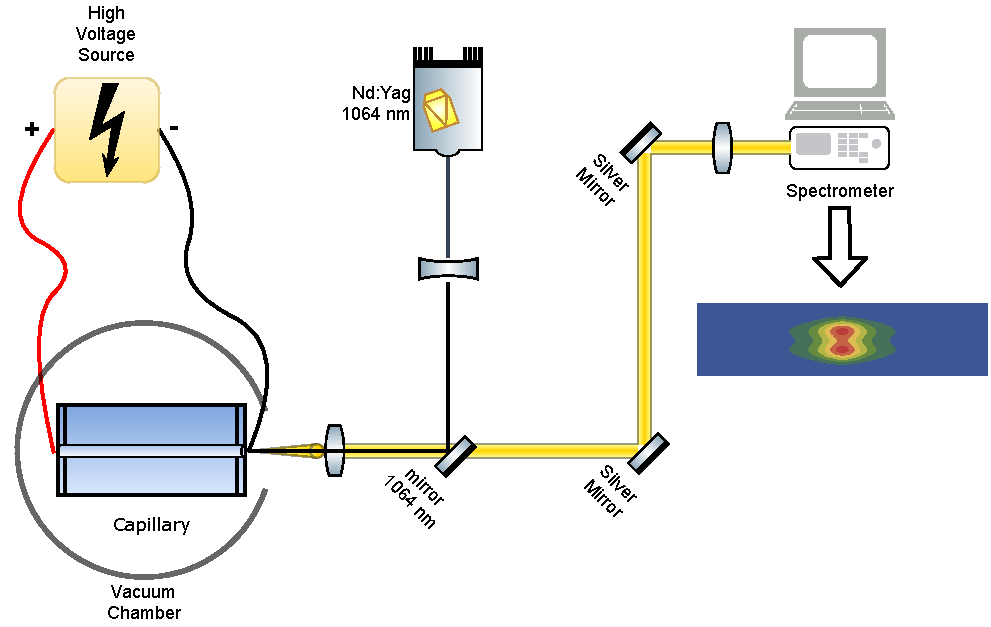
\includegraphics[height=152pt]{figures/results/spectro/radial_system.pdf}
 \end{figure}
Imaging system --- $\times 5$ magnification.

iCCD camera $\SI{40}{\ns}$ gate--on time. 

Width of the spectrometer slit --- \SI{150}{\um}.
\end{frame}
\begin{frame}{Spectroscopy Analysis}
\begin{figure}
\includegraphics[width=0.8\textwidth]{figures/results/spectro/spectra_analysis.png}
 \end{figure}
 pixel size = $\SI{26}{\um} \times \SI{26}{\um}$
\end{frame}
\begin{frame}{Spectroscopy Analysis}{cont.}
Fit a Lorentzian to each row of the data.
\tikzsetnextfilename{sample_lorentzian}
\begin{figure}
  \includegraphics[width=0.8\textwidth,height=160pt]{figures/results/spectro/sample_lorentzian.tikz}
\end{figure}
\vskip -1em
Stark Broadening on the order of \SI{3}{\nm}.
%% R square goodness of fit sim 0.813
\end{frame}
\begin{frame}{Spectroscopy measurements}{Radial density profile}
 {\small Density minimum on the axis of the capillary.}
 \begin{equation*}
\Delta N_e \sim \SI{4e17}{\per \cubic \cm}
 \end{equation*}
\begin{center}
 with $r_\text{ch}\approx \SI{50}{\um} \text{ and } N_e\left(0\right)\approx \SI{4e17}{\per\cubic\cm}.$
\end{center}
\tikzsetnextfilename{parabolic_profile}
\begin{figure}
\includegraphics[width=270pt,height=142pt]{figures/results/spectro/parabolic_profile.tikz}
\end{figure}
\end{frame}
\begin{frame}{Longitudinal density profile}{System setup}
\vskip -0.6em
{\small Verify longitudinal homogeneity of the plasma density.}
\begin{figure}
\includegraphics[height=160pt]{figures/results/spectro/longitudinal_system.pdf}
\end{figure}
The entire capillary length was imaged.

iCCD camera \SI{1}{\us} gate--on time.
\end{frame}
\begin{frame}{Longitudinal density profile}{Result}
Mean plasma density $\bar{N}_e$ of
\vskip -1em
$$ \bar{N}_e \sim \SI{3.3e17}{\per\cubic\cm}. $$
\vskip -2em
\tikzsetnextfilename{longitudinal}
\begin{figure}
\includegraphics[height=170pt,width=\textwidth]{figures/results/spectro/longitudinal.tikz}
\end{figure}
%% Doing the error analysis, I got N_e=3.3e17 plusminus 0.33e17 electrons per cubic cm.
\end{frame}
 
\subsection{Optical Guiding}
% \begin{frame}{Optical guiding}{System setup}
% System setup as before, but now adding an oscillator laser.
% 
% Pulses at a \SI{84}{\MHz} rate.
% \tikzset{external/export next=false}
% \begin{figure}
% \begin{tikzpicture}
%     \node[anchor=south west,inner sep=0] (image) at (0,0) {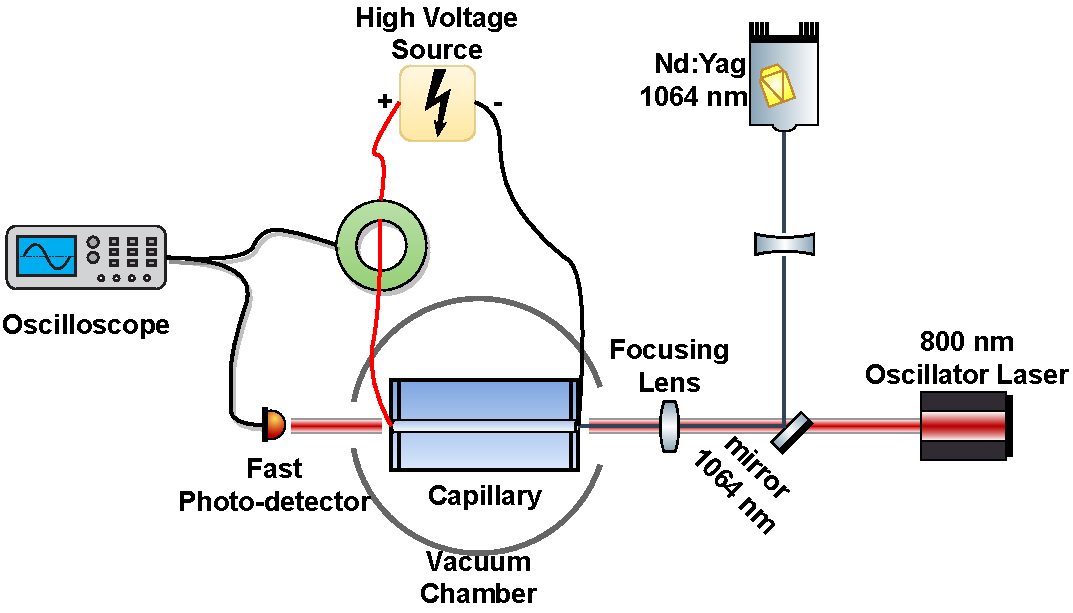
\includegraphics[height=140pt]{./figures/results/oscillator/oscillator_system_setup.pdf}};
%     \begin{scope}[xshift=230pt,yshift=76pt,scale=0.4]
% \begin{axis}[
%     width=260pt,
%     height=200pt,
%     grid=minor,
%     change x base,
%     x SI prefix=nano,
%     ytick=\empty,
%     xtick={-12.5e-9,0,12.5e-9,25e-9,37.5e-9,50e-9},
%     xmin=-20e-9,xmax=55e-9,
%     xlabel={Time [\si{\ns}]},
%     ylabel={Amplitude [\si{\volt}]},
%     label style={font=\Huge},
%     tick label style={font=\huge} 
%     ]
%     \addplot [red,line width=1pt] table[x=t,y=single,col sep=comma] {figures/results/oscillator/oscillator_waveform.csv};
% \end{axis}
%     \end{scope}
% \end{tikzpicture}
% \end{figure}
% Beam aligned through the capillary, to a fast photo--diode.
% \end{frame}
 
\begin{frame}{Optical Guiding}
Upon plasma discharge, we look for an increase in the

detected amplitude --- optical guiding.
\begin{equation*}
\text{transmission ratio} = \frac{A_{t<0}}{A_\text{max}}
\end{equation*}
The explanation:

A plasma lens forms, the radiation is focused and trapped by the plasma.
\begin{center}
 \includegraphics[width=0.6\textwidth]{figures/results/oscillator/chen_4_31.pdf}
\end{center}

\end{frame}

\begin{frame}{Optical guiding}{Results}
\tikzsetnextfilename{guiding01}
\vskip -2em
\begin{figure}
 \includegraphics[width=\textwidth,height=160pt]{figures/results/oscillator/guiding01.tikz}
\end{figure}

\vskip -1em
\fcolorbox{black}{ForestGreen}{\hspace{2mm}}\raisebox{-3pt}{ --- Nd:Yag laser pulse}

\fcolorbox{black}{blue}{\hspace{2mm}}\raisebox{-3pt}{ --- Rogowsky coil reading} \hskip 4em $\text{transmission ratio} \approx 2.1$

\fcolorbox{black}{red}{\hspace{2mm}}\raisebox{-3pt}{ --- detected oscillator signal}
\end{frame}

\begin{frame}{Optical Guiding}{results}
\tikzsetnextfilename{guiding02}
\begin{figure}
  \includegraphics[width=\textwidth,height=157pt]{figures/results/oscillator/guiding02.tikz}
\end{figure}
\vskip -1em
\fcolorbox{black}{ForestGreen}{\hspace{2mm}}\raisebox{-3pt}{ --- Nd:Yag laser pulse}

\fcolorbox{black}{blue}{\hspace{2mm}}\raisebox{-3pt}{ --- Rogowsky coil reading} \hskip 4em $\text{transmission ratio}= \frac{A_{t<0}}{A_\text{max}} \approx 8$

\fcolorbox{black}{red}{\hspace{2mm}}\raisebox{-3pt}{ --- detected oscillator signal}
\end{frame}
\begin{frame}{Duration of the plasma channel}
Correlation between applied voltage and the transmission ratio:
\tikzsetnextfilename{voltage_vs_guiding}
\begin{figure}
\includegraphics[width=0.5\textwidth,height=100pt]{figures/results/oscillator/voltage_vs_guiding.tikz}
\end{figure}
Duration of the plasma channel:
 \begin{equation*}
  \Delta t_\text{channel}=50 -100\ \si{\ns}.
 \end{equation*}
\end{frame}
% % \subsection{Two stage capillary}
% % \begin{frame}{Two stage capillary}
% %  As said in the introduction, a "fish--bone" capillary may overcome the dephasing length limitation.
% %    \begin{figure}
% %      \includegraphics[width=0.2\textwidth]{figures/theory/coupling_scheme.pdf}
% %    \end{figure}
% %    \begin{figure}
% %      \includegraphics[width=0.8\textwidth]{figures/results/2stageCapillary/doublecapillary_cad.png}
% %    \end{figure}
% %    2 stage, Y--shape capillary.
% % \end{frame}
% % \begin{frame}{Two stage capillary}{System setup}
% % \begin{figure}
% %     \includegraphics[width=\textwidth]{figures/results/2stageCapillary/setup.pdf}
% % \end{figure}
% % \end{frame}
% % \begin{frame}{Two stage capillary}
% % Split the oscillator pulse-–train to two beams, one for each capillary
% % channel.
% % Introduce a delay line to distinguish between each beam.
% % \begin{figure}
% %     \includegraphics[width=0.5\textwidth]{figures/results/2stageCapillary/double.png}
% % \end{figure}
% % \end{frame}
% % \begin{frame}{Results}
% % \begin{figure}
% % \includegraphics[width=0.8\textwidth]{figures/results/2stageCapillary/curved-pulsetrain-merged.png}
% % \end{figure}
% % \begin{columns}
% % \column{0.8\textwidth}
% % Note the "bump" of the signal recorded by the photo--diode.
% % 
% % To minimize this, use a screen to block as much unwanted light.
% % \column{0.2\textwidth}
% % \includegraphics[width=1\textwidth]{figures/results/2stageCapillary/opaquescreen.png}
% % \end{columns}
% % \end{frame}
\section{Summary}
\begin{frame}{Summary}
Study of plasma channels generated in gas filled--capillaries.

\begin{itemize}
\item Low jitter of discharge ignition
\item Verification of plasma conditions by spectroscopy means
\item Demonstration of optical guiding
\end{itemize}
Future experiments ---

Incorporating these capillaries in a LWFA scheme.

\end{frame}
% 
% % \begin{frame}{Double Capillary}{Results}
% % \tikzsetnextfilename{low_jitter_curved}
% % \begin{figure}
% %     \centering
% %     \includegraphics[width=\textwidth,height=142pt]{figures/results/doubleCapillary/low_jitter.tikz}
% % \end{figure}
% %     $$\tau_\text{jitter}\approx 1\pm 0.5\si{\ns}$$
% % \end{frame}
% % 
% % \begin{frame}{Double Capillary}{Results}
% % \tikzsetnextfilename{guiding01_double}
% % \begin{figure}
% %     \centering
% %     \includegraphics[width=\textwidth,height=142pt]{figures/results/doubleCapillary/guiding01_double.tikz}
% % \end{figure}
% % \end{frame}
% % \begin{frame}{Double Capillary}{Results}
% % \tikzsetnextfilename{guiding02_double}
% % \begin{figure}
% %     \centering
% %     \includegraphics[width=\textwidth,height=142pt]{figures/results/doubleCapillary/guiding02_double.tikz}
% % \end{figure}
% % \end{frame}
% % \begin{frame}{Wake waves}
% % \begin{columns}  
% % \column{0.5\textwidth}
% % \includegraphics[width=\textwidth]{figures/theory/boat_ski.jpg}
% % \column{0.5\textwidth}
% % \includegraphics[width=\textwidth]{figures/theory/boat_wake.jpg}
% % \end{columns}
% % \end{frame}
\end{document}